\documentclass[a4paper,11pt]{article} \usepackage[T1]{fontenc} \usepackage[utf8]{inputenc} \usepackage[francais]{babel}
\usepackage[top=2cm,left=2.5cm,right=2.5cm,bottom=2cm]{geometry} % Géométrie de la page, modifier selon le besoin
\usepackage{xcolor}
\usepackage{listingsutf8}
\usepackage{textcomp}
%\usepackage{minted}
\lstset{
    language=C++,
    keywordstyle=\bfseries\ttfamily\color[rgb]{0,0,1},
    identifierstyle=\ttfamily,
    commentstyle=\color[rgb]{0.133,0.545,0.133},
    stringstyle=\ttfamily\color[rgb]{0.627,0.126,0.941},
    showstringspaces=false,
    basicstyle=\small,
    numberstyle=\footnotesize,
    numbers=left,
    stepnumber=1,
    numbersep=10pt,
    tabsize=2,
    breaklines=true,
    prebreak = \raisebox{0ex}[0ex][0ex]{\ensuremath{\hookleftarrow}},
    breakatwhitespace=false,
    aboveskip={\baselineskip},
  columns=fixed,
  upquote=true,
  extendedchars=true,
  inputencoding=utf8/latin1
}


\lstset{language=C++}
\usepackage{lmodern, wrapfig, textcomp, tikz, graphicx}





\begin{document}
\begin{titlepage}
%
\includegraphics[scale=0.45]{Images/logo_phelma.pdf}\hfill
\begin{center}
    \vspace*{1cm}
    \textsc{\Large Bureau d'Études d'Informatique}\\
    [4.5cm] \rule{\linewidth}{0.5mm}\\[0.4cm]
    {\huge\bfseries Fractales et FLTK\\
    [0.4cm]}\rule{\linewidth}{0.5mm}\\[1.0cm]
    \textsc{pmpB}
    \begin{flushright} \large
        % \emph{Entrepreneurs :} \\
        Julia \textsc{Dupuis}\\
        Nils \textsc{Exibard}\\
        Félix \textsc{Piédallu}\\
    \end{flushright}
    
    
  \begin{center}
    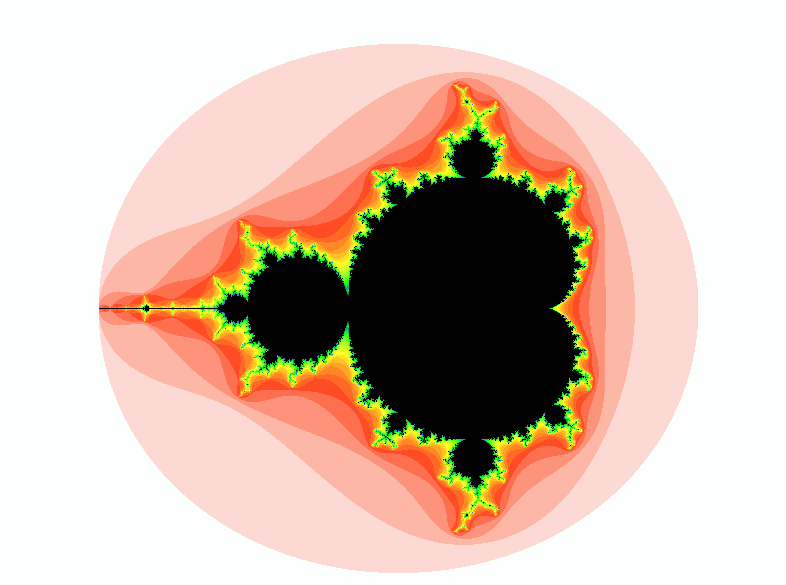
\includegraphics[width=0.7\textwidth]{Images/Titlepage.png}
  \end{center}

    \vfill

    \large{\today}
\end{center}
\end{titlepage}
     % Fichier de page de titre
\tableofcontents          % Table des matières avec liens, générée automatiquement.
\vspace{3cm}
%\input{0.Intro.tex}       % Fichier d'intro, à mettre ici peut-être
\newpage

\section{Présentation du programme}
Le sujet  sur lequel nous avons choisi de travailler est le projet « Fractales », grand classique de la programmation, utilisant le plan complexe.
%\begin{figure}[h] \begin{center} 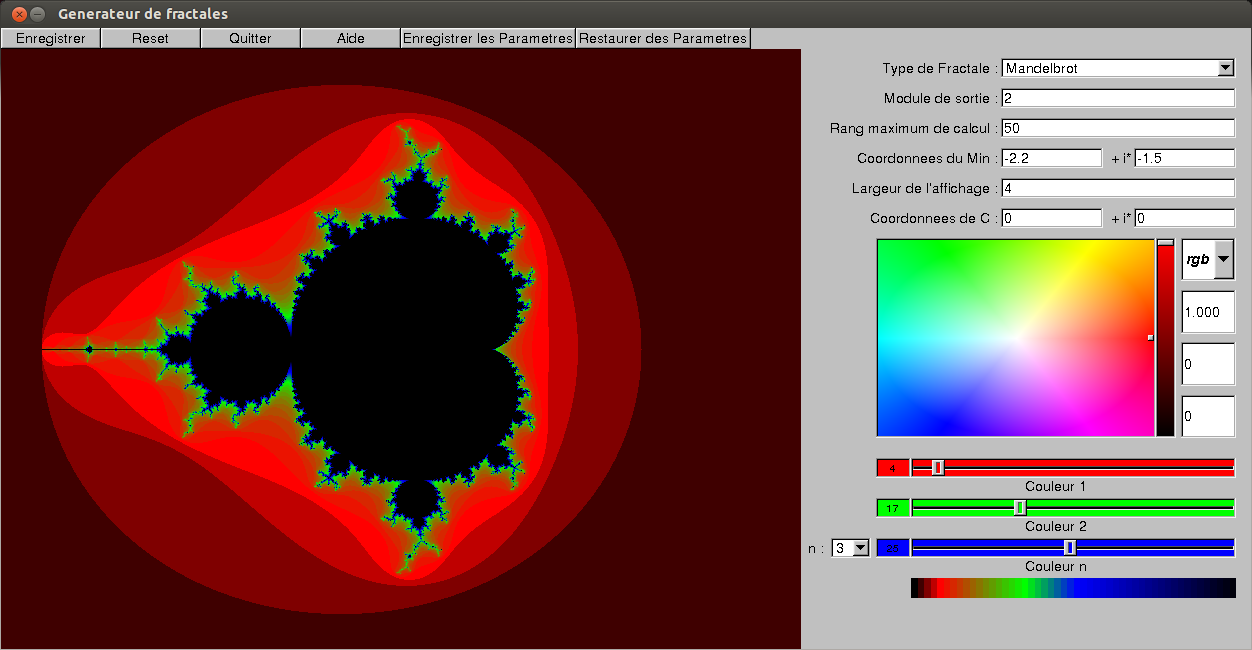
\includegraphics[width=\textwidth]{Images/InterfaceTotale}
    %\caption{}
%\end{center} \end{figure}

Les fonctionnalités que nous avons choisi d'intégrer sont les suivantes :
\begin{itemize}
  \item Calcul et tracé dans la zone de dessin de 4 types de fractales (Mandelbrot, Julia, sin, cos). %image à changer, le type personna n'y est plus (pull and see)
    %    \begin{figure}[h]  \begin{center} \includegraphics[width=0.5\textwidth]{Images/ChoixFractale.png}
        %    \caption{}
        %\end{center} \end{figure}
  \item Choix par l’utilisateur des différents paramètres de la fractale (type, module de sortie, rang maximal, coordonnées du point inférieur gauche, largeur de l’affichage, coordonnées de la constante).
        %\begin{figure}[h] \begin{center} 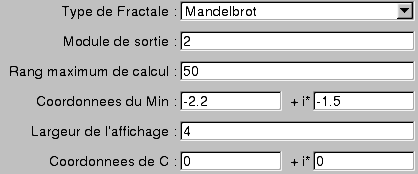
\includegraphics[width=0.5\textwidth]{Images/Parametres.png}
            %\caption{}
        %\end{center} \end{figure}
  \item Choix des couleurs (jusqu'a 10 couleurs choisies par l’utilisateur avec écart modifiable). %image à changer
        %\begin{figure}[h] \begin{center} \includegraphics[width=0.5\textwidth]{Images/ChoixCouleur.png}
            %\caption{}
        %\end{center} \end{figure}
  \item Enregistrement de l’image ainsi que des paramètres dans un fichier choisi par l’utilisateur avec une qualité choisie.
  \item Restauration de paramètres précédemment enregistrés.
  \item Remise à zéro des paramètres (bouton reset).
  \item Fonction « Quitter ».
  \item Un bouton aide expliquant les fonctionnalités des différents boutons de la souris.
        %\begin{figure}[h] \begin{center} 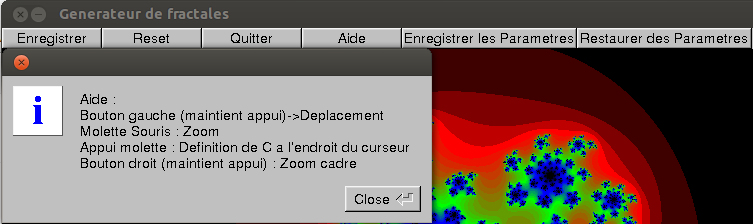
\includegraphics[width=0.5\textwidth]{Images/Aide.png}
           % \caption{}
        %\end{center} \end{figure}
  \item 2 types de zoom : avec cadre(clic droit) ou grâce à la molette .
        %\begin{figure}[h] \begin{center} \includegraphics[width=0.5\textwidth]{Images/ZoomBox.png}
            %\caption{}
        %\end{center} \end{figure}
  \item Déplacement de l’image (clic gauche maintenu).
\end{itemize}

\section{Sources}
\subsection{Structures de données}
\begin{lstlisting}
struct Pixel {
    complex<double> z;      //Coordonnées du pixel dans le plan complexe
    int n;                  //Rang de divergence du pixel
};
Cette strcure permettra de tracer la fractale à partir du rang de divergence et de la coordonnée de chaque pixel
\end{lstlisting}
\begin{lstlisting}
struct Donnees {
    enum fractype Fractale; // Type de fractales choisie (Type énuméré)
    int     rangMax;        // Rang maximal de convergence
    double  moduleMax;      // Module de convergence (determination de la convergence on non de la fonction)
    complex<double> C;      // Constante de calcul
    complex<double> ig;     // Coordonnees du point inferieur gauche
    double pasxy;           // Pas de la matrice (incrementation, en fait, et egale dans les 2 dimensions, car pixels carres)
    struct Pixel Tab[L_ZONE][H_ZONE]; // Matrice des pixels de l'image.
int hauteur;             //Hauteur de l'image
    unsigned char buffer[3*L_ZONE*H_ZONE];//contient l'image sous forme RGB
    unsigned char bufferDeg[3*325];//contient l'apperçu du dégradé sous forme RGB
    int nbSlider;           //Nombre de slider actifs
    unsigned long int slider[MAX_SLIDER+2][2];//contient le rang et la couleur de chaque slider
};

\end{lstlisting}
Cette structure est la plus importante du programme.

\begin{lstlisting}
struct Tests {
    bool dessin;//faut-il refaire le dessin?
    bool calcul;//faut il refaire le calcul
    bool calccouleurs;//faut il refaire le calcul des couleurs ?
    int slider; //contient le slider actif
};
\end{lstlisting}
Cette structure contient les variables nécessaires à la vérification des conditions, cela permet entre autre d’éviter les calculs inutiles.

\begin{lstlisting}
enum fractype {
    MANDELBROT,
    JULIA,
    COSC,
    SINZO,
    PERSONNA//Originellement prévue pour une fractale personnalisée, non utilisée faute de temps
};
\end{lstlisting}
Le type énuméré permet d’utiliser plus facilement les différents types de fractales.


\subsection{Fonctions }
\begin{lstlisting}
void InitialiserDonnees() ;
\end{lstlisting}
Initialise les données du programmes
\begin{lstlisting}
void realFromTab(double *bi, double *bj);
\end{lstlisting}
Effectue la correspondance entre les coordonnées complexe et les pixels
\begin{lstlisting}
pointeurFct retourne_fonction();    // Pointe vers les fonctions suivantes en fonction de la fractale choisie
\end{lstlisting}
%Félix t'expliqueras ça probab mieux que moi
\begin{lstlisting}
int mandelbrot(complex<double> position);
int julia     (complex<double> position);
int sinzo     (complex<double> position);
int cosc      (complex<double> position);
int personna  (complex<double> position);
\end{lstlisting}
Ce sont les algorithmes de calcul de convergence
\begin{lstlisting}
void convergenceLigne(int j, pointeurFct fonction);
\end{lstlisting}
Etudie la convergence ligne par ligne
\begin{lstlisting}
void degradeRGB(unsigned long int A, unsigned long int  B,int N, int tab[][3]);
\end{lstlisting}
Effectue le calcul d'un dégradé de taille N entre une couleur A et une couleur B, et stocke les trois composantes RGB dans tab
\begin{lstlisting}
void couleursRGB(unsigned long tabSlider[][2],int tab[][3]) ;
\end{lstlisting}
Remplis tab d'une suite de dégradé grace à degradeRGB à partir des informations contenues dans tabSlider
\begin{lstlisting}
void calcBuffer(int tabdeg[][3]);
\end{lstlisting}
calcule et stocke dans gDonnees.bufferDeg a partir d'un tableau de couleurs RGB
\begin{lstlisting}
int enregistrerPPM(int Largeur, char Fichier[32]);
\end{lstlisting}
Enregistre une image en ppm de Largeur pixel de large et de ratio constant dans Fichier.
\begin{lstlisting}
void enregistrerParams(const char* fichier);
void restaurerParams(const char* fichier);
\end{lstlisting}
Permet d'enregistrer (et de lire, mais non finalisé) les paramètres permettants de redéssiner la fractale

\subsection{Affichage}
\begin{lstlisting}
void ZoneDessinInitialisation(Fl_Widget* widget, void* data);
\end{lstlisting}
%Initialise la zone de dessin puis appelle gestionAffichage_iter
\begin{lstlisting}
void afficheFractaleLigne();
\end{lstlisting}
Commande le calcul puis l'affichage d'une ligne
\begin{lstlisting}
void afficheLigneRGB(int j, int tableauCouleurs[][3]);
\end{lstlisting}
Affiche la ligne j avec pour couleurs un tableau RGB
\begin{lstlisting}
void gestionAffichage_iter(void* data);//iter car en remplacement de la fonction récursive d'origine.
\end{lstlisting}
Calcule SI nécéssaire la fractale puis l'affiche grace aux diverses autres fonctions.
\begin{lstlisting}
void tracerCadre (int x1, int y1 , int x2, int y2);
\end{lstlisting}
Trace le cadre du zoom cadre a partir de 2 points (conserve le ratio d'écran)
\begin{lstlisting}
void zoneDegrade(Fl_Widget* widget, void* data);
\end{lstlisting}
Gère l'affichage de la zone d'apperçu du dégradé



\section{Critique}
\section{Déroulement du projet}
\begin{lstlisting}
#ifndef _Main_h
#define _Main_h
#include <FL/Fl_Widget.H>

class DrawingArea : public Fl_Widget{
public:
    DrawingArea(int X,int Y,int W,int H);
    void draw_callback( void (*Function) (Fl_Widget* w, void* data), void* Data);
    void mouse_callback( void (*Function) (Fl_Widget* w, void* data), void* Data);
    void keyboard_callback( void (*Function) (Fl_Widget* w, void* data), void* Data);

private :
    void draw();
    int handle(int event);

    void (*_draw_callback_function) ( Fl_Widget* w, void* data);
    void* _draw_callback_data;

    void (*_mouse_callback_function) ( Fl_Widget* w, void* data);
    void* _mouse_callback_data;

    void (*_keyboard_callback_function) ( Fl_Widget* w, void* data);
    void* _keyboard_callback_data;
};
#endif

\end{lstlisting}

\end{document}
